\documentclass{beamer}
\setbeamertemplate{navigation symbols}{}

\usepackage{beamerthemeshadow}
\usepackage{graphicx}
\usepackage{url}
\usepackage{listings}

\begin{document}
\title{Stackbased Languages}
\author{Serap Kadam, Christoph M{\"u}llner \\
$<$serapkadam@gmail.com$>$, $<$christophm30@gmail.com$>$
}
\subtitle{Knight's Tour}

\date{\today} 

\begin{frame}
\titlepage
\end{frame}

\begin{frame}
\frametitle{Table of contents}
\tableofcontents
\end{frame} 

\section{Knight's tour} 
\begin{frame}
\frametitle{The problem}
The Knight's Tour is a mathematical problem involving a knight
on a chessboard. The knight is placed on the empty board and,
moving according to the rules of chess, must visit each square
exactly once.

In German this problem is called "Springerproblem".
\end{frame}

\begin{frame}
\frametitle{Variations of the knight's problem}
\begin{itemize}
	\item Find a path for a given start/end position
	\item Find a closed path for a given position
	\item Find a path for a board of size $n x m$
\end{itemize}
\end{frame}

\subsection{Background}
\begin{frame}
\frametitle{The knight and his movement}
\begin{figure}
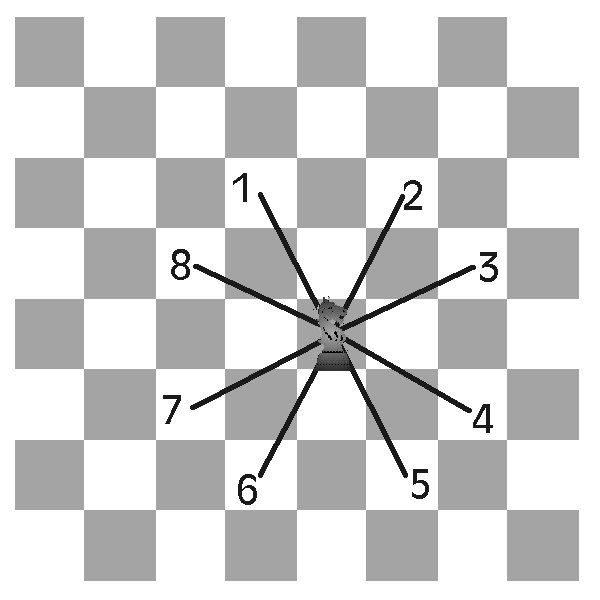
\includegraphics[scale=0.25]{sprung}
\caption{Possible moves of a knight}
\end{figure}
\end{frame}

\subsection{Solutions}
\begin{frame}
\frametitle{Backtracking}
\begin{itemize}
	\item Choose an unvisited position
	\item Backtracking if no unvisited position reachable
\end{itemize}
\end{frame}

\begin{frame}
\frametitle{Warnsdorff's algorithm}
\begin{itemize}
	\item Choose unvisited position, which has the fewest successor positions
	\item Only a (very good) heuristic => must not find a solution
	\item Found by H. C. Warnsdorff (1823)
\end{itemize}
\end{frame}

\begin{frame}
\frametitle{Other solutions}
\begin{itemize}
	\item For bigger boards: D\&C
\end{itemize}
\end{frame}

\section{Implementation}
\subsection{Language, task description}
\begin{frame}
\frametitle{Language and task description}
\begin{itemize}
	\item Language: PostScript (Ghostscipt)
	\item Input: End position of knight
	\item Output: Path of knight to end position
	\item Completeness for $8 x 8$ boards
\end{itemize}
\end{frame}

\end{document}
